\chapter{Design and Implementation of KadPeer}
\label{chap3}
{
The architecture design was done according to the effort paied to the study of the issues that addressed.
A lot of time has been spent on the project was used to study a possible solution of \emph{OGG} file spliting and merging.
I obtained the simplest possible method to the spliting policy using the characteristics of containers and codecs of \emph{OGG}.

To obtain the P2P integration the quality streams will be encapsulated into a metadata file which was inspired from the design of BitTorrent.
The metadata will contain the infomation of the ordinary stream and also extra track infomation which is used for initiating the decoder.
However, my P2P related design does not depend on the BitTorrent but \emph{kademlia} ,the decentralized structure infrastructure.

At first sight it was clear that the only way to go was to exploit the possibility of assigning media chuncks to different peers of a metadata to be able to download the part by not lossing pages of stream. As we are going to see later this feature is the heart of scheduler controller which enable to downlaod the chuncks with correct order.
}

\section{Overall Design Precept Description}
{

The \emph{KadPeer} aims at the \emph{VoD} services which provides high performance of video playing includes audio and captions as well, and also allows users search the video content he/she interested.
And the features list as followed:
\begin{itemize}
\item Login and logout the network system. (basic, but GUI interface is optional and it will be future task)
\item Interface to publish the media data. (basic)
\item Search the media resource that the users might be interested.(basic)
\item List up the known resource in the internet.(basic)
\item Play the Video that user select from the known resource list or search result.(basic)
\item Jump forwards and jump backwards of video on playing arbitrarily.(basic)
\item Download the video resource directly from the search result.(optional)
\item Tranfer data through NAT or firewalls.(optional)
\end{itemize}

In allusion to the features list above, I gave out the related design ideas and the resolvent.
The chart below illustrates the global structure of \emph{KadPeer}.
\begin{center}
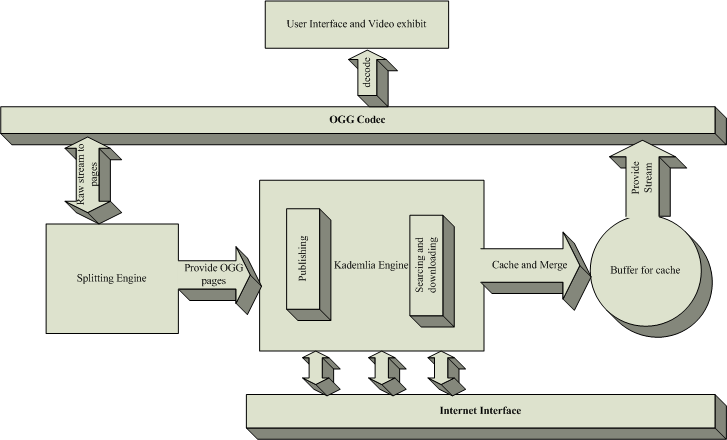
\includegraphics[width=15cm]{data/KadPeerStructure.png}
\end{center}
As we can see from the above chart, there are two important engines in KadPeer.
One is kademlia related which handles the backend video distributed and swarming, the other is video data operation related which handles video content parsing and provides basic infomation for OGG codec to do video splitting.

To implement \emph{KadPeer}, I have anaylsed and take the usage of more than 10 librarys which covered the important functions of the client, such as thrift, libogg, libtheora, libvorbis,libkate, and oggplayer.
I will select some of the important librarys to illustrate how these third part librarys worked in kadpeer later.
}

\subsection{Important Third Part Libs and the Integration}
\subsubsection{Thrift}
{
Thrift is a software library and set of code-generation tools developed at Facebook to expedite development and implementation of efficient and scalable backend services. 
Its primary goal is to enable efficient and reliable communication across programming languages by abstracting the portions of each language that tend to require the most customization into a common library that is implemented in each language.

Specifically, Thrift allows developers to define datatypes and service interfaces in a single language-neutral file and generate all the necessary code to build RPC clients and servers.

The base types supported by Thrift are:
\begin{itemize}
\item \texttt{bool} A boolean value, true or false
\item \texttt{byte} A signed byte
\item \texttt{i16} A 16-bit signed integer
\item \texttt{i32} A 32-bit signed integer
\item \texttt{i64} A 64-bit signed integer
\item \texttt{double} A 64-bit floating point number
\item \texttt{string} An encoding-agnostic text or binary string
\item \texttt{binary} A byte array representation for blobs
\end{itemize}
Also, Thrift defines a common object to be used across languages. 
A struct is essentially equivalent to a class in object oriented programming languages. 
A struct has a set of strongly typed fields, each with a unique name identifier. 
The basic syntax for defining a Thrift struct looks very similar to a C struct definition. 
%Fields may be annotated with an integer field identifier (unique to the scope of that struct) and optional default values.

In KadPeer, for the kademlia engine implementation, RPC related functions are based on the Thrift library.
Additional structs of thrift has been defined in kadpeer such as ``ContactInfo'',''signed\_kadvalue'' and ``kademila messages'', in which the exchange data are contained during the communication process.

%Thrift reduces the effort that I should pay for on the 
}

\subsubsection{libogg,liboggz,libtheroa,libvorbis,libkate}
{
%The librarys listed above are \emph{OGG} container.
Oggz provides a simple programming interface for reading and writing Ogg files and streams. Ogg is an interleaving data container developed by Monty at \emph{Xiph.Org}, originally to support the Ogg Vorbis audio format.
Support is built-in for parsing the headers of and seeking to time positions in Ogg Dirac, FLAC, Speex, Theora and Vorbis. 
Oggz is also compatible with Annodex streams, and supports seeking on all tracks described in an Ogg Skeleton track.

Theora is a general purpose, lossy video codec. It is based on the VP3 video
codec produced by On2 Technologies (http://www.on2.com/). 
On2 made an irrevocable, royalty-free license grant for any patent claims it might have over the software and any derivatives. 
Theora contains a superset of the features that were available in the original
VP3 codec. Content encoded with VP3.1 can be losslessly transcoded into the
Theora format.\cite{THEORA}

The Vorbis audio CODEC provides a channel coupling mechanisms designed to reduce effective bitrate by both eliminating interchannel redundancy and eliminating stereo image information labeled inaudible or undesirable according to spatial psychoacoustic models.
In encoder release beta 4 and earlier, Vorbis supported multiple channel encoding, but the channels were encoded entirely separately with no cross-analysis or redundancy elimination between channels. This multichannel strategy is very similar to the mp3's dual stereo mode and Vorbis uses the same name for its analogous uncoupled multichannel modes.\cite{VORBIS} 

Kate is an overlay codec, originally designed for karaoke and text, that can be multiplixed in Ogg. Text and images can be carried by a Kate stream, and animated. Most of the time, this would be multiplexed with audio/video to carry subtitles, song lyrics (with or without karaoke data), etc, but doesn't have to be.
Series of curves (splines, segments, etc) may be attached to various properties (text position, font size, etc) to create animated overlays. This allows scrolling or fading text to be defined. This can even be used to draw arbitrary shapes, so hand drawing can also be represented by a Kate stream.\cite{KATE}
}

\subsubsection{liboggplay}
{
\begin{center}
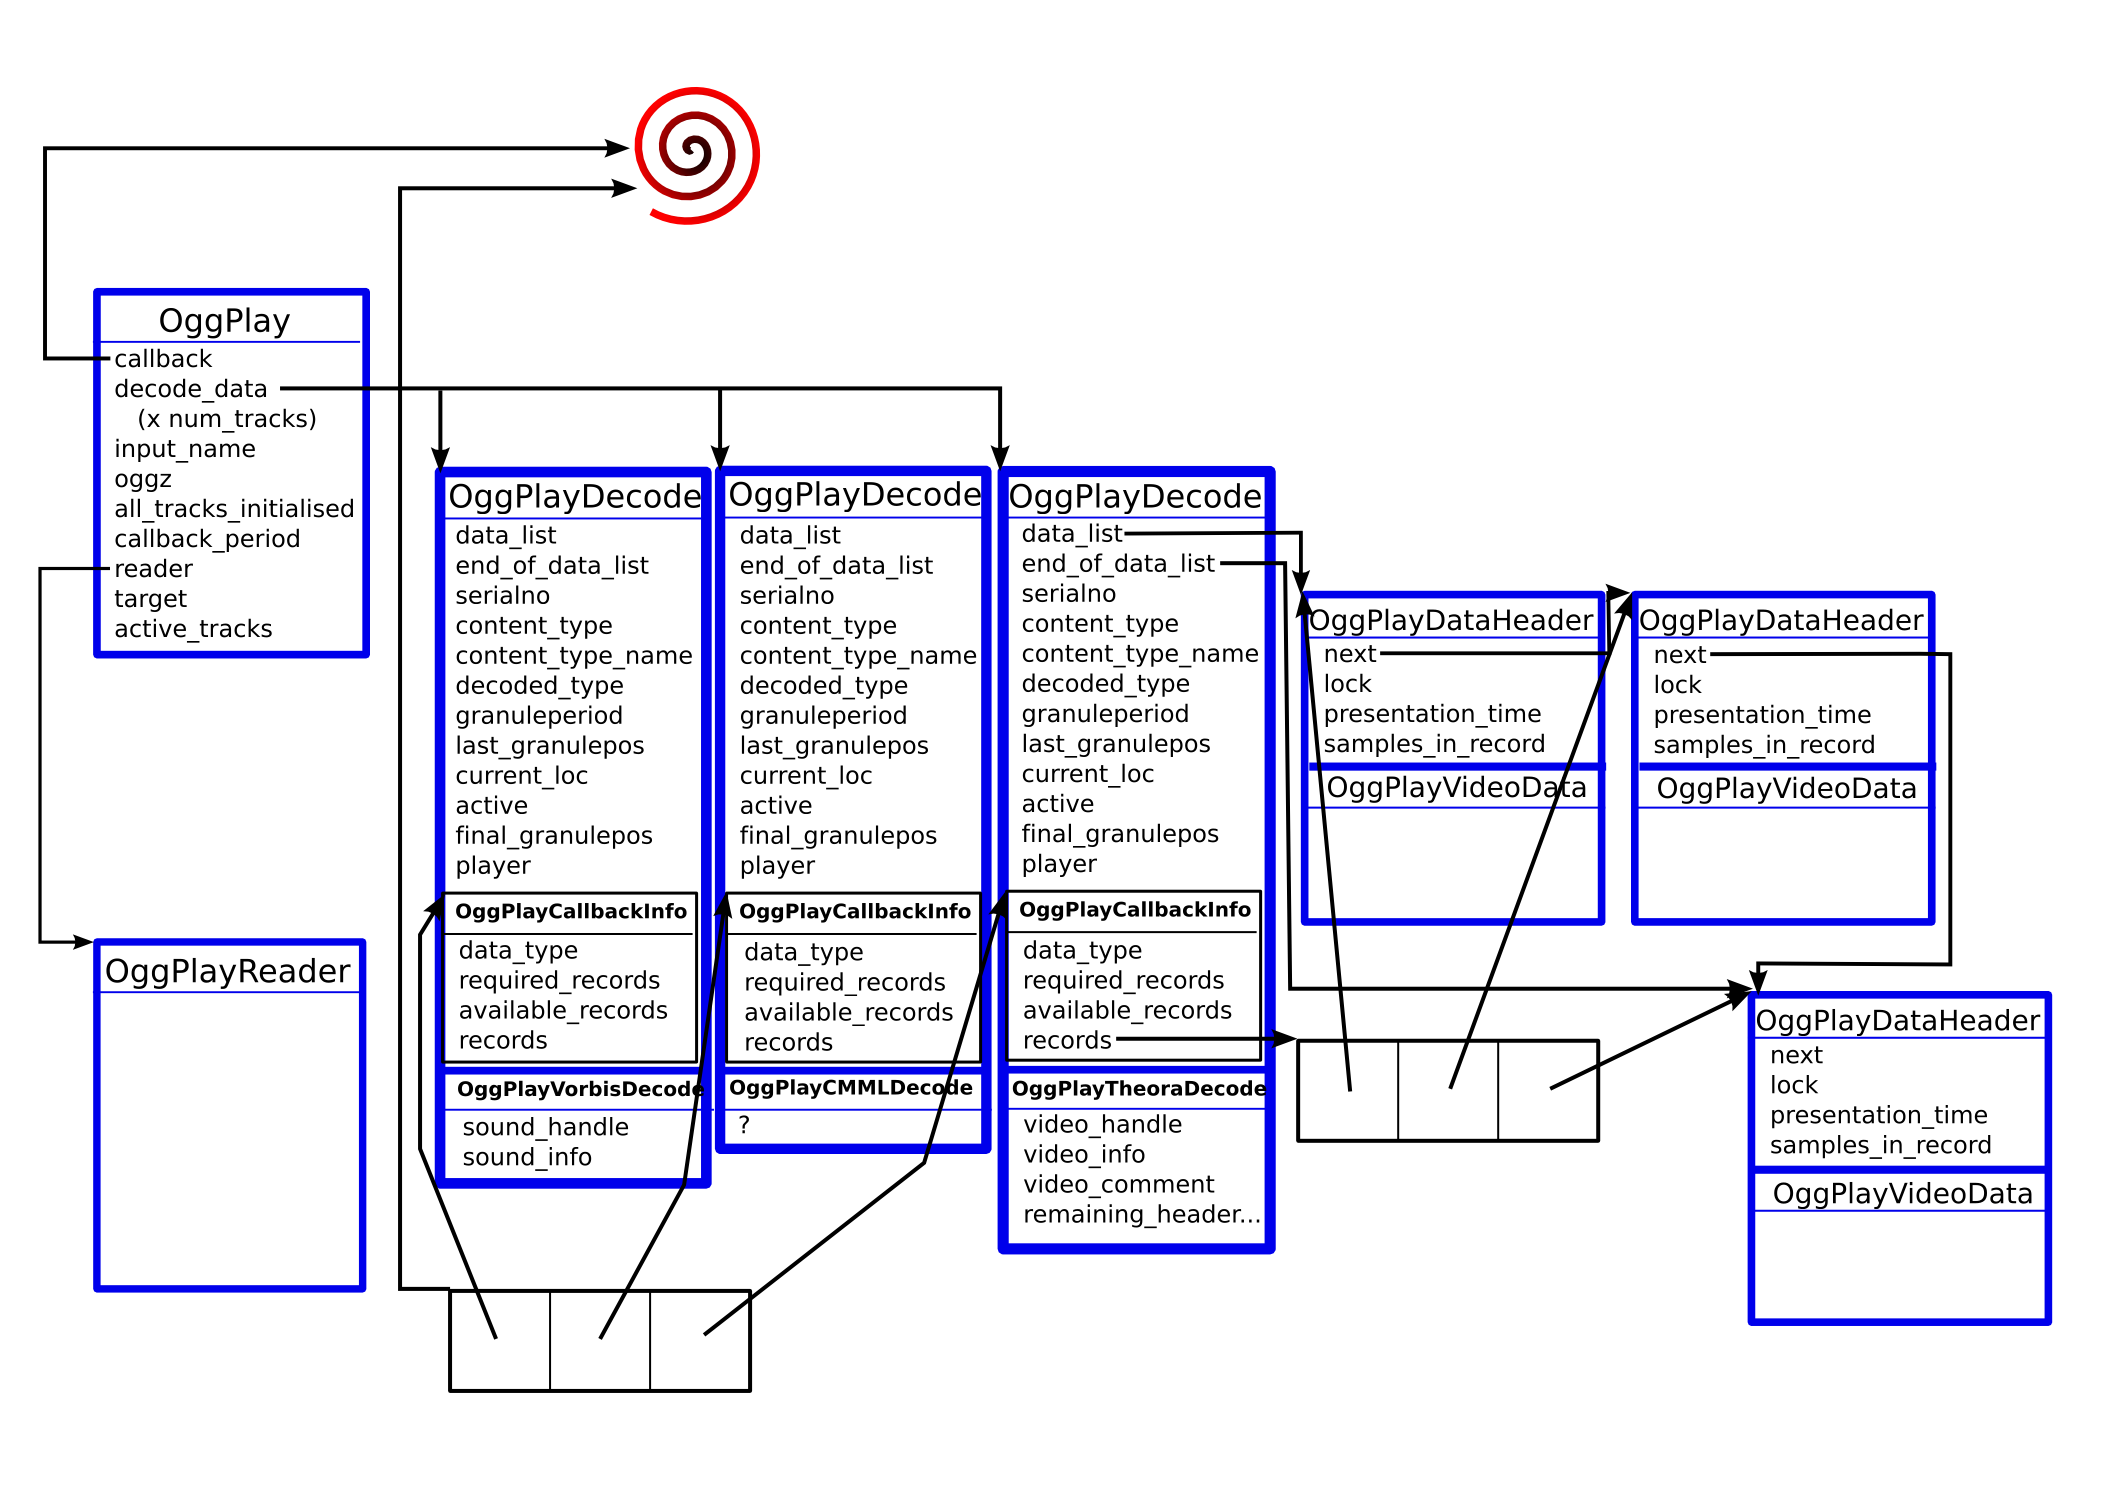
\includegraphics[width=15cm]{data/liboggplay_data_layout.png}
\end{center}
}

\subsection{Meatadata Format}
{
The problem of how to produce a metadata infomation according to the specify video stream was the first to be addressed.
Because of its big importance in the project. it has been considered from various points of view.

Let us review the torrent mechanism used in BitTorrent liked system. 
Torrent file is the most important part of the whole BT system, which includes the infomation of Tracker server and the the segments to download. 
We can consider the torrent file is the carrier of BitTorrent protocol. When using the BT to download a related file, you have to get the torrent file first.
Torrent file contains the basic infomation of the file to download, such as file name, file size, and location infomation of the file publisher server.
So, the BitTorrent client can search the server according to the infomation that torrent file provided.
At the end, an extra \emph{SHA1} checksum to ensure the integrality and validity of the segment.

what to be highlighted is the codec format of torrent file which was so-called "Bencode".
“Bencode" infomation contains string, dictionary and nestification of list.

The "Bencode" data structures are as followed:

%\begin{center}
\begin{tabular}{|l|c|l|}\toprule
Types      &  Express Mode                           & Sample  \\ \midrule
string     &  \textless length\textgreater :context  & 4:spam \\ \hline
Integer    &  \textless i\textgreater integer\textless e\textgreater          & i3e means decimal 3 \\
           &                                         & i-3e means decimal -3 \\ \hline
List       &  \textless i\textgreater Bencode Value\textless e\textgreater & l4:spam4:eggse \\
           &                                          &        means \\
          &                                            & ['spam','eggs'] \\ \hline  
Dictionary & \textless d\textgreater \textless Bencode String\textgreater \textless Bencode element\textgreater \textless e\textgreater &d3:cow3:moo4:spam4:eggse \\
        &                                       &means \\
           &                                         &   {'cow':'moo','spam':'eggs'}\\
\bottomrule
\end{tabular}
%\end{center}

A torrent file is a bencoded dictionary with the following keys:
\begin{itemize}
\item announce - the URL of the tracker
\item info - this maps to a dictionary whose keys are dependent on whether one or more files are being shared:
\begin{itemize}
\item name - suggested file/directory name where the file(s) is/are to be saved
\item piece length - number of bytes per piece. This is commonly 2$^{18}$ = 256KiB = 262144B.
\item pieces - concatenation of each piece's SHA-1 hash. As SHA-1 returns a 160-bit hash, pieces will be a string whose length is a multiple of 160-bits.
\end{itemize}
\end{itemize}

% And exactly one of length (corresponds to when only one file is being shared) or files (corresponds to when multiple files are being shared):
% \begin{itemize}
% \item length - size of the file (in bytes)
% \item files - a list of dictionaries (each dictionary corresponds to a file) with the following keys:
% \item path - a list of strings corresponding to subdirectory names, the last of which is the actual file name
% \item length - size of the file (in bytes)
% \end{itemize}
%All strings must be UTF-8 encoded.

As I have introduced the \emph{OGG format} in the begining of my thesis. 
Ogg file has different attributes compared with the other format files, so we can mux the design of BitTorrent to create new format of metadata infomation which can be used efficiently to manage the resource in the DHT environment.

However, I did not follow the ``Bencode'' format completely, great changes were committed to the design of metadata format.
\begin{enumerate}
\item Athough the ``bencode'' has been an easy way for encoding and parsing the content of a torrent file, I did not continue to use ``becode''. 
It was because I intended to combine more complex data format in the metadata info. And moreover, this new kinds of format should be more convenient to  transfer to string, we need to deliver the string on the internet arbitrarily. 
I take up \emph{XML} -- the structured language to mantian the metadata, which has been implemented by many opensource developers.
The most famous project which implements the \emph{XML} with C plus plus programming language is \emph{tinyxml} on sourceforge\cite{tinyxml}. 
The \emph{Tinyxml} has provided simple and convenient APIs to make it easily integrating into other programs, especially this XML parser is lightweight, stable and constructed with STL( when compiling , you should add special definitions to compile options to enbale STL.)which makes this integration more compact, because the \emph{KadPeer} is constructed with pure C++ in \emph{Linux } platform.
%TinyXML is a simple, small, C++ XML parser that can be easily integrating into other programs.
\item The elements to record the video file in metadata which users published or shared on the internet were changed compaired with the torrent components. 
I add additional infomation to the metadata such as track numbers among the \emph{Theora, Vorbis and Kate} streams that the video file might contain, the theroa stream rates, the samplerates and channels of the Vorbis stream, the language and category of Kate stream, and extra comments that the user might want to mark the video resource.
These additail infomation formulates the video file in a quantize way which also provides enough content to the stream decoder and validates the page head that the scheduler swarmed from the internet.
\item The content for recording each splited chuncks is still \emph{SHA1}.
There are two reasons for this obtainment. 
First,\emph{SHA1} of the chuncks could be used as the identifier of the specify chunk.
Secondly, the output of \emph{SHA1} is 160B, of which the length is equal to that of  node ID in \emph{kademlia}.
That means in the process of distribution, we can directly assgin specify node to store the video chunck with specify SHA1 output and in the process of swarming, we also use the SHA1 output to gether the chuncks we needed.
\end{enumerate}

%A sample XML content of metadata is as fowlloed:
%\lstinputlisting[frame=tb]{metadata.xml}
}

\subsection{Spliting and Scheduler}
{
In the design of BitTorrent, the piece of each chunck is 2$^{18}$ B which has been provided as a good performance on chunck spliting and distribution. 
However, as the \emph{OGG} stream is orgnized with pages which header\_size = number\_page\_segments  + 27 [Byte] and page\_size = header\_size + sum (lacing\_values:1...number\_page\_segments)[Byte].
so I decide to splite the stream with size as near as that of BT.
And for another reason, all types of track (Theroa,Vorbis,Kate) are multiplexed in one OGG stream which are encapsulated by page.
Thanks for the design of the tracks, We do not have to pay more effort to reoganize the three tracks or dump each of them and reencapsulate them.
The follow chart illustrates the multiplexing process of multipule logical bitstreams to one physical bitstream.

\begin{center}
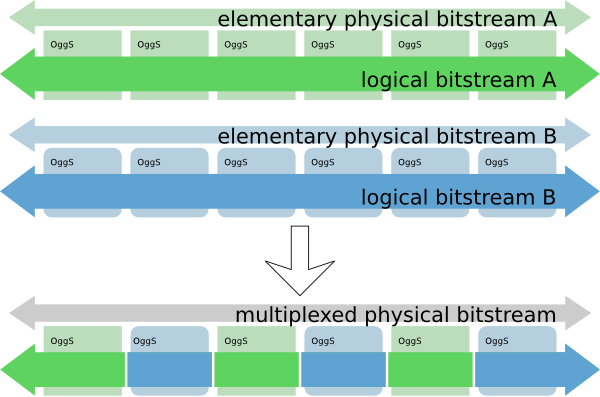
\includegraphics[width=8cm]{data/multiplex1.png}
\end{center}

The max size of a physical page is nearly 2$^{14}$ B, compared to 2$^{18}$ B of BT chunck.
So I define the granularity of spliting interval is 2$^{4}$ = 16 pages each chunck.
In general, the size of each chunks is dynamic, cause the size of each page are different, but 16 pages will buildup a typical chunck. However, no matter what the size of each chunck is, the SHA-1 of chunck data is always 160 B, that is the trick point of the design.

Refer to the infrastructure of metadata I provided before, after parsing the meta content, the SHA-1 value of each chunck will be stored in both a vector and buffer map.
After the vector was initalize,the content of the vetor would be constant, espically the order of the vector.
Because the order of vector should be the original order of video file spliting, we need to refer to the vector to recompse the \emph{OGG} bitstream.
The usage of the buffer map is to store the chuncks that low level swarming engine gethered from the internet.

}

\subsection{Buffer and Cache}
{
Usually the resource to feed codec is stored on the local disk which can be easily randomly accessed by the read function provided by system call with a simple API.
I have anaylsed the implementation of \emph{OGGPlayer} deeply.
While reading flat video file in local disk, there is a buildin ring buffer to store the data for synchronization.

The data structure of the buffer showed as followed:
\begin{lstlisting}[frame=tb]{}
typedef struct {
  void   ** buffer_list;
  void   ** buffer_mirror;
  int       buffer_size;
  int       last_filled;
  int       last_emptied;
  semaphore frame_sem;
} OggPlayBuffer;
\end{lstlisting}
In the buffer construction phase, the two level pointer ``buffer\_list will alloc a appointed size, the iterator last\_filled and 

%The buffer with a default size 20 B which 

\begin{center}
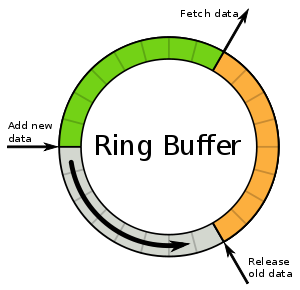
\includegraphics[width=5cm]{data/Ringbuffer.png}
\end{center}  

}

